\section{Existing Solutions Sufficient?}
\label{sec:existing}
In this section, we explore the third question: are existing network-layer solutions sufficient to meet the requirements imposed by the applications in \dis? We start by describing the methodology (\S\ref{ssec:ssmethod}), and then evaluate the network-level (\S\ref{ssec:nlp}) and application-level performance (\S\ref{ssec:alp}) in \dis using existing network-level solutions.

\subsection{Methodology}
\label{ssec:ssmethod}
We explore the sufficiency of existing network-layer solutions for \dis in two steps. First, we take the flows generated from \S\ref{sec:workloads} and simulate the network-layer performance (flow completion time) for these flows. We then return to our emulator, take the respective flow completion time for flows, and inject the respective latencies using SIT, as described in \S\ref{sec:requirements}, thus allowing us to evaluate the application level performance. 

For all the simulations in this section, we use the setup from prior work in datacenter transport simulation~\cite{pfabric, phost}. In particular, we simulate a $144$-node full bisection bandwidth fat-tree topology with $40$Gbps access link capacity. \rc{What else do we need to describe?} However, there are multiple challenges in executing the above two steps that we had to resolve.

\paragraphb{Scaling up}
\begin{enumerate}
\item our data is for 5 ec2 nodes, but we have a 144-node topology to fill.
\item the 5 ec2 nodes map to 5 cpu blades, 5 memory blades, and 3 disk blades
\item so in our 13-node trace we collect a interarrival and size CDF per s-d pair
\item for each node in the 144, we assign it a sender profile and pick 12 other nodes as destinations
\item the interarrival and flow size cdfs for flows between a source and destination as picked in the previous step are used to generate flows.
\item this should give an idea of network loads in a full-dc disaggregated scenario from a transport perspective.
\end{enumerate}

\paragraphb{Level of disaggregation: $3\times$ problem?}
\begin{enumerate}
\item before, one "blade" had 3 resources - cpu, memory, disk
\item now, each "blade" has only one resource
\item so, each blade should have 3x of its assigned resource
\item the flow generation from above is run 3x for each node.
\end{enumerate}

\paragraphb{Latency injection for long flows}
\begin{enumerate}
\item blktrace does not intercept, it only logs
\item we cannot inject latency into disk access
\item this is okay because a. memory is more latency sensitive anyway 
\item and b. there are more memory flows than disk flows.
\item accordingly we only consider the slowdown distribution of memory flows when injecting.
\end{enumerate}

\subsection{Network-level performance}
\begin{enumerate}
\item Figure~\ref{fig:phostp} shows network transport performance.
\item we use the mean slowdown metric used by pFabric and phost~\cite{pfabric, phost}.
\item the takeaway is that performance is near-optimal for both.
\item we conclude that existing transport protocols are sufficient because:
\item \rqc{reasons}
\end{enumerate}
\label{ssec:nlp}

%
\begin{figure}
  \centering
    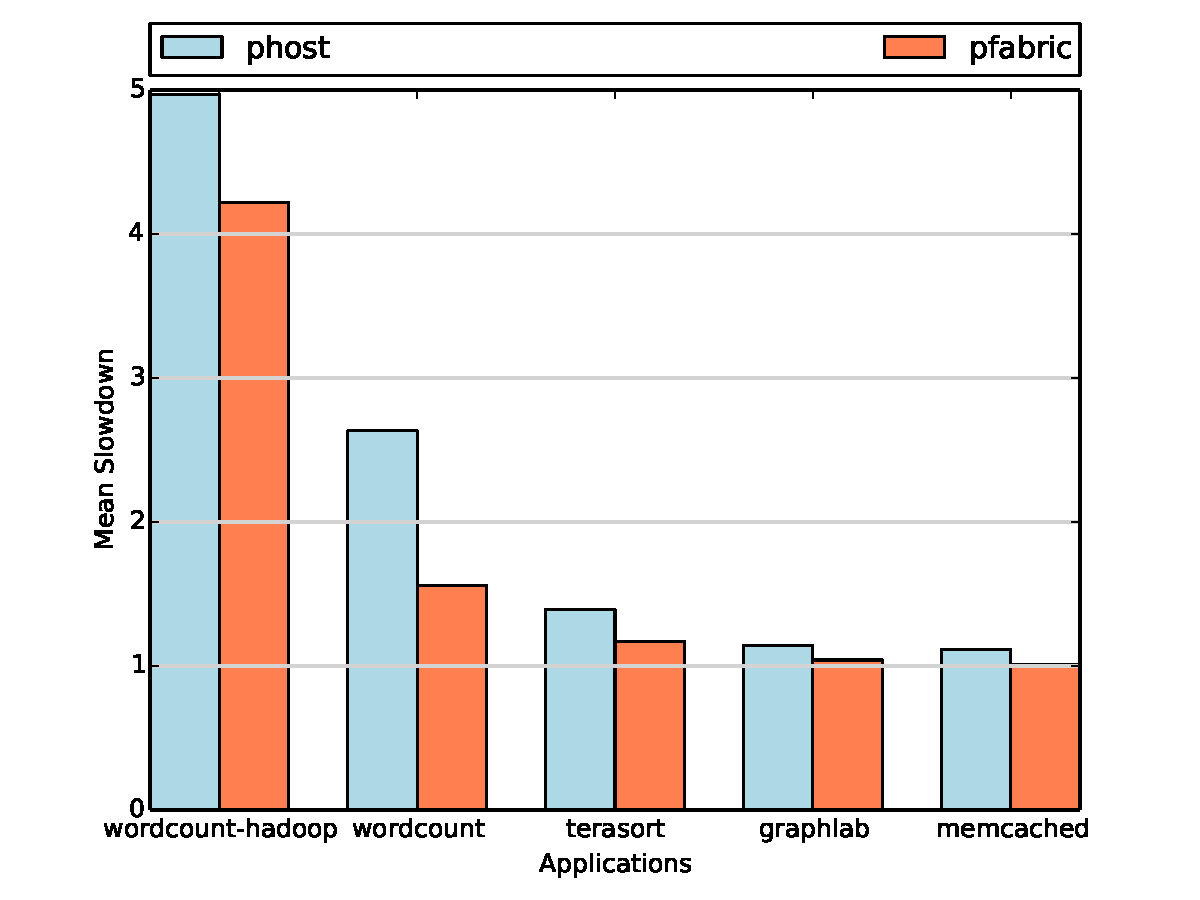
\includegraphics[width = 2.5in]{img/fig12_slowdownsGraph} 
  \caption{\small{The mean slowdown for pFabric and pHost for each of the six applications. \rc{(remove phost?)}}}
  \label{fig:phostp}
\end{figure}
%

\subsection{Application-level performance}
\label{ssec:alp}

%
\begin{figure}
  \centering
    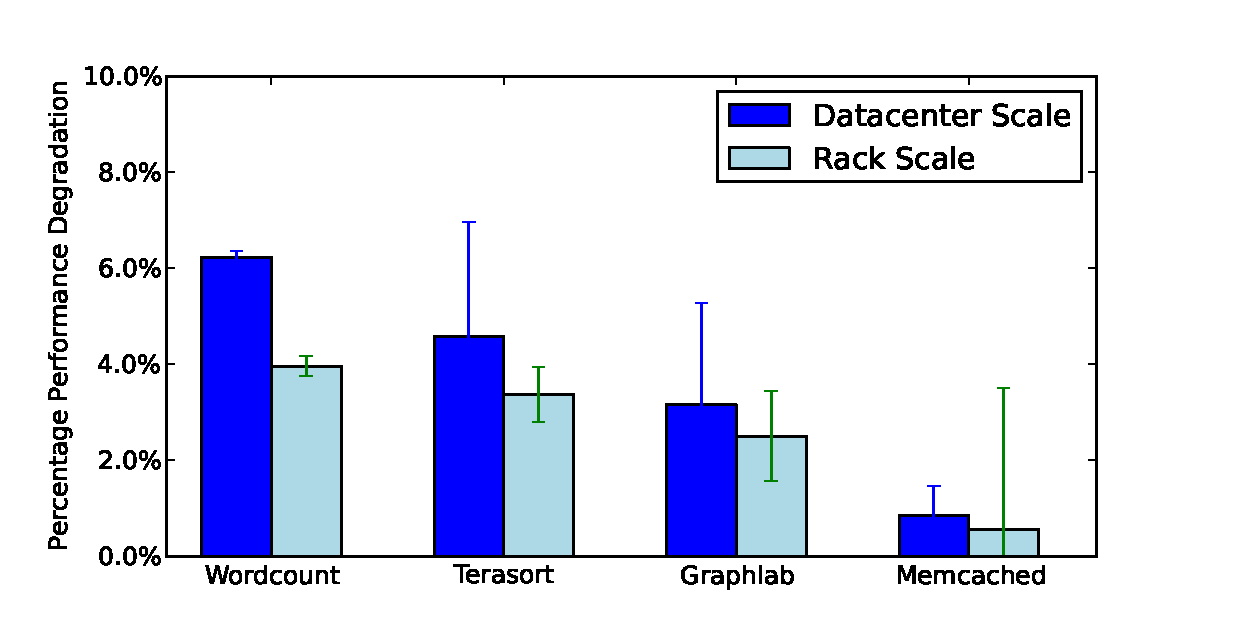
\includegraphics[width = 2.5in]{img/slowdown.eps} 
  \caption{\small{\rqc{Application layer slowdown for each of the six applications.}}}
  \label{fig:appfabric}
\end{figure}
%
